\subsubsection{Comparing Direct form II and J-Look-Ahead}
What will be presented now is an analysis of the data obtained from the two filters, with the aim of demonstrating their equivalence in behavior despite the great difference between the two topologies. In particular they will be examined in Matlab environment:

\begin{itemize}
	\item Initial signal values
	\item Average of the two signals
	\item Variance of the two signals
\end{itemize}

Notice that the IIR look-ahead filter topology in \autoref{the figure} has two pipeline stages between the input and output signal, this implies that the signal has a higher latency than the Direct form II topology, which corresponds exactly to two clock cycles. The table in \autoref{fig:THD_table} shows the results of the two implementations.

\begin{figure}[ht]
	\begin{minipage}[b]{0.5\linewidth}
		\centering
		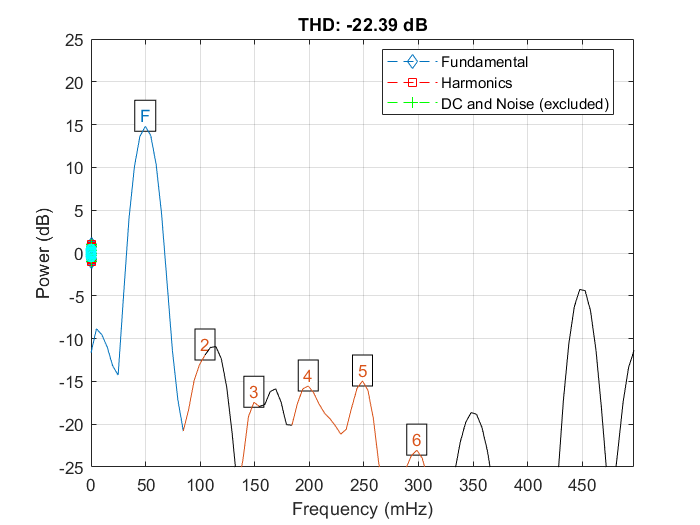
\includegraphics[width=\textwidth]{JLAH_THD_5_bit_C_result.png}
		\caption{THD of IIR J-Look-Ahead filter}
		\label{fig:THD_5_bit_IIR_JLA}
	\end{minipage}
	\hspace{0.5cm}
	\begin{minipage}[b]{0.4\linewidth}
		\centering
		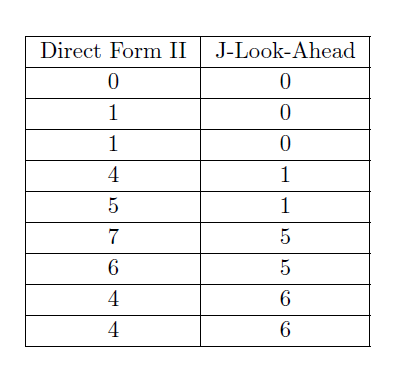
\includegraphics[width=\textwidth]{THD_table.png}
		\caption{Results of the two implementations compared}
		\label{fig:THD_table}
	\end{minipage}
\end{figure}

As the J-look-Ahead {THD} graph has anticipated, the two signals are not perfectly identical in the values and although the overall trend may be very similar, one may be interested in how different it actually is, so an analysis of the output signals from the two qualitative and quantitative filters is necessary at this point. Afterwards, the average and variance values of the two signals are represented:

\begin{table}[H]
	\begin{center}
		\begin{tabular}{|c|c|c|}
			\hline
			Parameter		& Direct Form II	& J-Look-Ahead 			\\ \hline
			Mean			&$-0.8308$  		& $-2.2537$	           	\\ \hline
			Variance		&$23.6312$      	& $32.9303$             \\ \hline
			
		\end{tabular}
	\end{center}
\end{table}

The two signals are not perfectly identical, and in fact they present different averages and variance, but they have the same order of magnitude and values consistent with the system under analysis. For a finer analysis it is necessary to use Allan's variance to measure how much the noise degrades the performance and how much the oscillatory behavior of the output is more or less stable. In \autoref{fig:Allan_Var_DF2} the variance of the two signals is represented and in \autoref{fig:Allan_Var_difference} the difference between the two variance to assess how much the stability of Direct Form II differs from that of J-Look-Ahead, both graphs were generated using the Matlab function \textit{allanvar()}:

\begin{figure}[ht]
	\centering
	\begin{minipage}[b]{0.44\linewidth}
		\centering
		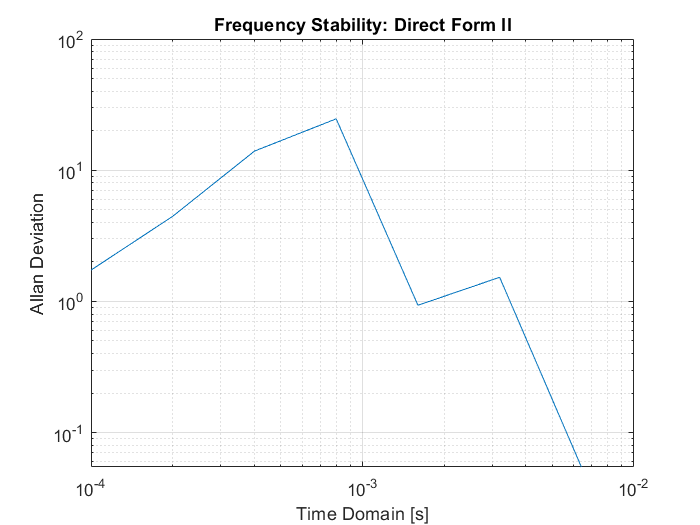
\includegraphics[width=\textwidth]{Allan Var DF2.png}
		\caption{Allan variance of the Direct Form II  and J-look-ahead IIR Filter}
		\label{fig:Allan_Var_DF2}
	\end{minipage}
	\hspace{0.5cm}
	\begin{minipage}[b]{0.48\linewidth}
		\centering
		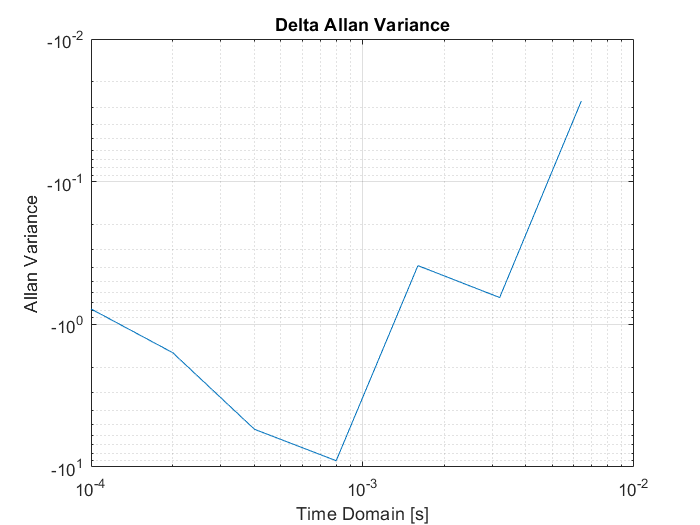
\includegraphics[width=\textwidth]{Allan Var difference.png}
		\caption{Difference of the 2 Allan variance}
		\label{fig:Allan_Var_difference}
	\end{minipage}
\end{figure}